
\documentclass[a4paper,12pt]{article}
%%%%%%%%%%%%%%%%%%%%%%%%%%%%%%%%%%%%%%%%%%%%%%%%%%%%%%%%%%%%%%%%%%%%%%%%%%%%%%%%%%%%%%%%%%%%%%%%%%%%%%%%%%%%%%%%%%%%%%%%%%%%%%%%%%%%%%%%%%%%%%%%%%%%%%%%%%%%%%%%%%%%%%%%%%%%%%%%%%%%%%%%%%%%%%%%%%%%%%%%%%%%%%%%%%%%%%%%%%%%%%%%%%%%%%%%%%%%%%%%%%%%%%%%%%%%
\usepackage{eurosym}
\usepackage{vmargin}
\usepackage{amsmath}
\usepackage{graphics}
\usepackage{epsfig}
\usepackage{subfigure}
\usepackage{fancyhdr}
%\usepackage{listings}
\usepackage{framed}
\usepackage{graphicx}

\setcounter{MaxMatrixCols}{10}
%TCIDATA{OutputFilter=LATEX.DLL}
%TCIDATA{Version=5.00.0.2570}
%TCIDATA{<META NAME="SaveForMode" CONTENT="1">}
%TCIDATA{LastRevised=Wednesday, February 23, 2011 13:24:34}
%TCIDATA{<META NAME="GraphicsSave" CONTENT="32">}
%TCIDATA{Language=American English}

\pagestyle{fancy}
\setmarginsrb{20mm}{0mm}{20mm}{25mm}{12mm}{11mm}{0mm}{11mm}
\lhead{MA4128} \rhead{Mr. Kevin O'Brien}
\chead{Advanced Data Modelling}
%\input{tcilatex}


% http://www.norusis.com/pdf/SPC_v13.pdf
\begin{document}
	
	
	%SESSION 1: Hierarchical Clustering
	% Hierarchical clustering - dendrograms
	% Divisive vs. agglomerative methods
	% Different linkage methods
	
	%SESSION 2: K-means Clustering
	
	\tableofcontents
	\newpage




The hierarchical clustering procedure attempts to identify relatively homogeneous groups of cases (or variables) based on selected
characteristics. For example: cluster television shows into homogeneous groups based on viewer
characteristics. In hierarchical clustering, an algorithm is used that starts with each case (or variable) in a
separate cluster and combines clusters until only one is left.



To cluster cases you need to identify variables you wish to be considered in creating clusters for the cases.
The variables to be used for cluster formation are here: picture quality (5 measures), reception quality (3
measures), audio quality (3 measures), ease of programming (1 measure), number of events (1 measure),
number of days for future programming (1 measure), remote control (3 measures), and extras (3 measures).
Pass these in the Variable(s) box.

Cluster Method: Choose the procedure for combining clusters. The default procedure is called the
between-group linkage. SPSS computes the smallest average distance between all group pairs and
combines the two groups that are closest. The procedure begins with as many clusters as there are cases
(here: 21). At step one, the two cases with the smallest distance between them are clustered. Then SPSS
computes distances once more and combines the two that are next closest. After the second step you will
have either 18 individual cases and one cluster of 3 cases, or 17 individual cases and two clusters of two
cases each. The process continues until all cases are grouped into one large cluster.
Measure: Indicate what method is used for distance measuring, the default is Squared Euclidean distance. 

\subsection{Linkage methods}
\begin{itemize}
	\item  Single linkage (minimum distance)
	\item  Complete linkage (maximum distance)
	\item  Average linkage
\end{itemize}

%http://www.rdg.ac.uk/~aes02mm/supermarket.sav

\subsubsection{Ward's method}
\begin{itemize}
	\item  Compute sum of squared distances within clusters
	\item  Aggregate clusters with the minimum increase in the
	overall sum of squares
\end{itemize}
\subsubsection{Centroid method}
The distance between two clusters is defined as the
difference between the centroids (cluster averages)

\begin{itemize}

\item A commonly used approach in hierarchical clustering is \textbf{\textit{Ward’s linkage method}}.
This approach does not combine the two most similar objects successively. Instead,
those objects whose merger increases the overall within-cluster variance to the
smallest possible degree, are combined. If you expect somewhat equally sized
clusters and the data set does not include outliers, you should always use Ward’s
method.

We will use the Ward's linkage method for laboratory exercises.

\item Other most popular
agglomerative clustering procedures include the following:
\begin{description}
	\item[Single linkage (nearest neighbor)]: The distance between two clusters corresponds
	to the shortest distance between any two members in the two clusters.
	\begin{figure}[h!]
		\begin{center}
			% Requires \usepackage{graphicx}
			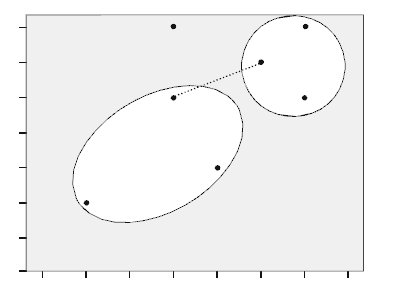
\includegraphics[scale=0.4]{images/Link1.jpg}\\
		\end{center}
	\end{figure}
	\item[Complete linkage (furthest neighbor)]: The oppositional approach to single
	linkage assumes that the distance between two clusters is based on the longest
	distance between any two members in the two clusters.
	\begin{figure}[h!]
		\begin{center}
			% Requires \usepackage{graphicx}
			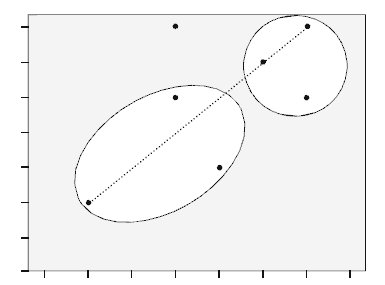
\includegraphics[scale=0.4]{images/Link2.jpg}\\
		\end{center}
	\end{figure}
	\item[Average linkage] : The distance between two clusters is defined as the average
	distance between all pairs of the two clusters’ members.
	\begin{figure}[h!]
		\begin{center}
			% Requires \usepackage{graphicx}
			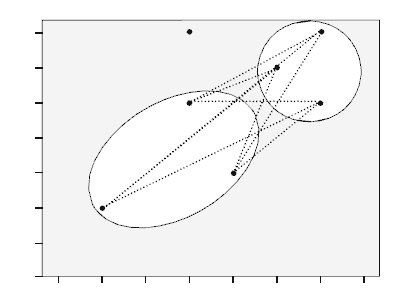
\includegraphics[scale=0.4]{images/Link3.jpg}\\
		\end{center}
	\end{figure}
	\newpage
	\item[Centroid] : In this approach, the geometric center (centroid) of each cluster is
	computed first. The distance between the two clusters equals the distance between
	the two centroids.
	\begin{figure}[h!]
		\begin{center}
			% Requires \usepackage{graphicx}
			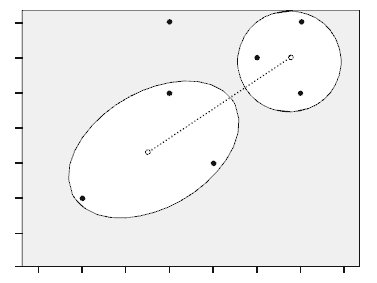
\includegraphics[scale=0.4]{images/Link4.jpg}\\
		\end{center}
	\end{figure}
\end{description}
Each of these linkage algorithms can yield totally different results when used on the same data set, as each has its specific properties. As the single linkage algorithm is based on minimum distances, it tends to form one large cluster with the other clusters containing only one or few objects each. We can make use of this \textbf{\textit{chaining effect}} to detect outliers, as these will be merged with the remaining objects – usually at very large distances – in the last steps of the analysis. Generally, single linkage is considered the most versatile algorithm.

Conversely, the complete linkage method is strongly affected by outliers, as it is based on maximum distances. Clusters produced by this method are likely to be rather compact and tightly clustered. The average linkage and centroid algorithms tend to produce clusters with rather low within-cluster variance and similar sizes.
However, both procedures are affected by outliers, though not as much as complete linkage.

An understanding of linkage method's other than than Ward method will be expected in the end of year examination.

\item A common way to visualize the cluster analysis’s progress is by drawing a
dendrogram, which displays the distance level at which there was a combination
of objects and clusters.
Here is an example of a dendrogram (which corresponds to the example in the next section of material.


\begin{figure}[h!]
	\begin{center}
		% Requires \usepackage{graphicx}
		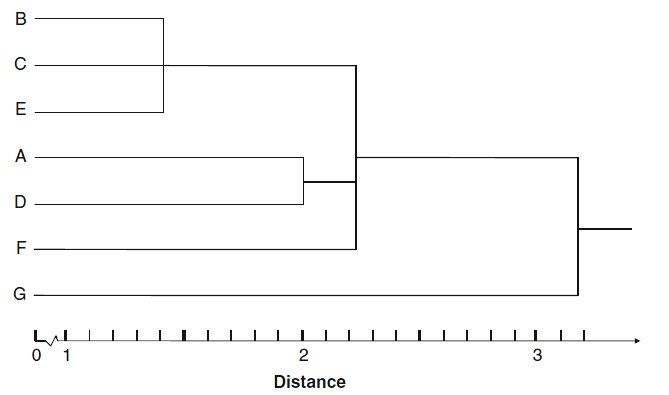
\includegraphics[scale=0.6]{images/Dendrogram.jpg}\\
	\end{center}
\end{figure}

\item An important question is how to decide on the number of
clusters to retain from the data. Unfortunately, hierarchical methods provide only
very limited guidance for making this decision. The only meaningful indicator
relates to the distances at which the objects are combined. Similar to factor
analysis’s scree plot, we can seek a solution in which an additional combination
of clusters or objects would occur at a greatly increased distance. This raises the
issue of what a great distance is, of course. For this purpose, we can make use of the dendrogram.

\item In constructing the dendrogram, SPSS rescales the distances to a range
of 0–25; that is, the last merging step to a one-cluster solution takes place at a
(rescaled) distance of 25. The rescaling often lengthens the merging steps, thus
making breaks occurring at a greatly increased distance level more obvious.
Despite this, this distance-based decision rule does not work very well in all
cases.

It is often difficult to identify where the break actually occurs. This is also
the case in our example above. By looking at the dendrogram, we could justify
a two-cluster solution ([A,B,C,D,E,F] and [G]), as well as a five-cluster solution
([B,C,E], [A], [D], [F], [G]).


\item 
The clustering algorithm is based on a distance measure that gives the best results if all variables are independent, continuous variables have a normal distribution (or categorical variables have a multinomial distribution). This is seldom the case in practice, but the algorithm is thought to behave reasonably well when the assumptions are not met.

\item 
Because cluster analysis does not involve hypothesis testing and calculation of observed significance levels, other than for descriptive follow-up, it's perfectly acceptable to cluster data that may not meet the assumptions for best performance.
\item 
The final outcome may depend on the order of the cases in the file. To minimize the effect, arrange the cases in random order. Sort them by the last digit of their ID numbers or something similar.
\end{itemize}
\end{document}